\subsection{Captain of the guards}

\begin{minipage}{0.5\textwidth}
\textbf{Function}:Chief of the guards, rules his subjects and runs the jail

\subsubsection{Internal World}

\textbf{Age \& Gender}: 50, Male \\
\textbf{Values \& Virtues}: Loyal to the queen\\
\textbf{Ethnic Group}: Human/Demon

\subsubsection{External World}
\textbf{Environment}: Castle of Dynamia \\
\textbf{Look \& Feel}: Tall, big and fat man\\
\textbf{Type of attack}:Melee and ranged \\
\end{minipage}%
%
\hfill\begin{minipage}{0.4\textwidth}
  \begin{figure}[H]
  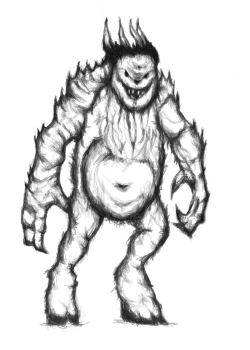
\includegraphics{Images/Enemies/captain_portrait}
   \caption{Sketch of the captain made by Elena Coperchini}
  \end{figure}
\end{minipage}


\subsubsection{Description and background story}
The captain was, without any doubt, the strongest and scariest man who ever joined the guards and due to this Mizar has chosen him for one of her experiments. Given his extreme faith, loyalty and submission to the queen, the captain immediately accepted her offer and so Mizar blended him with one of her demons making him even stronger, scarier and faster, gifting him also a new magic pistol.

